\chapter{VSD}
\begin{figure}[h]
\centering
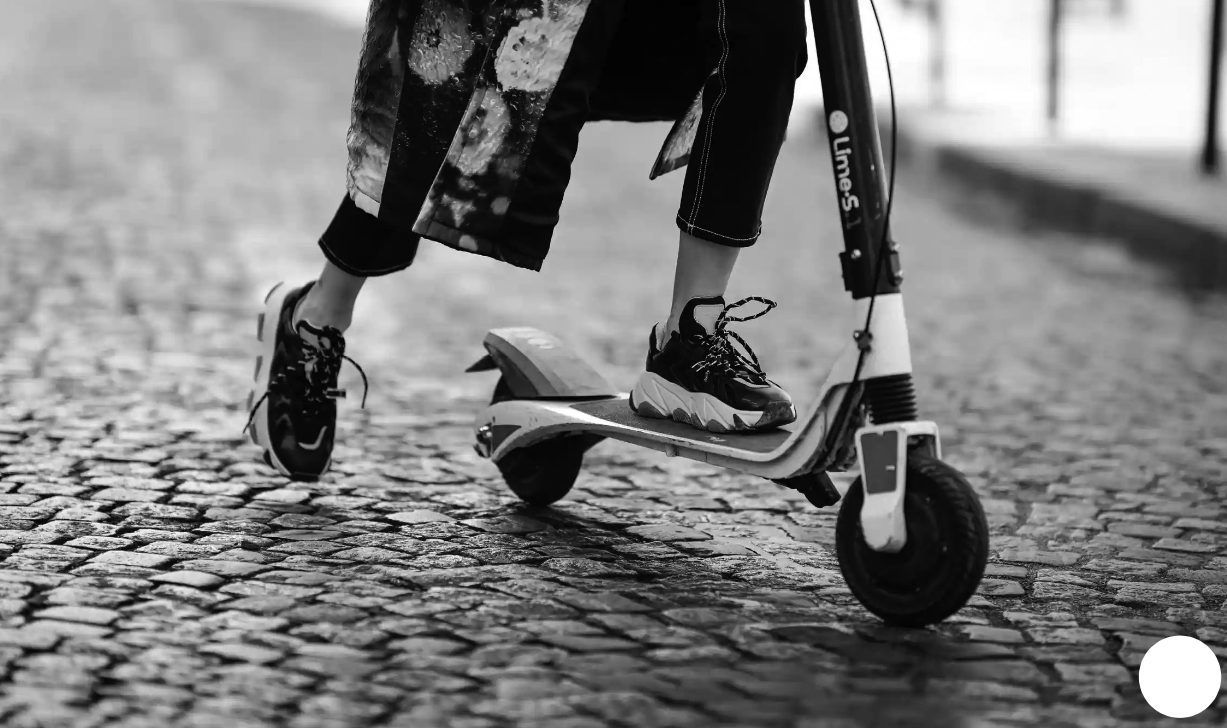
\includegraphics[width=0.8\textwidth]{Capitoli_Report/2.1_VSD.png}
\caption{\cite{vsdpic}}
\label{fig:vsd}
\end{figure}
\newpage
\pagestyle{plain}
\section{Introduction}
The case study regards the problem of e-scooters in urban context, critically reviewed using the \textit{Value Sensitive Design} method seen during the lesson. The stakeholder we selected is a \textit{pedestrian}, and we chose safety \textit{safety} as a value.

In the next table are listed the selected value, the norms and their design requirements:

\begin{table}[h]
\centering
\begin{tabular}{|l|l|l|}
\hline
\multicolumn{1}{|c|}{\textbf{Value}} & \textbf{Norms}                           & \textbf{Design requirements}        \\ \hline
\multirow{8}{*}{Safety}              & \multirow{2}{*}{Road rules}              & Use of separate lane                \\ \cline{3-3} 
                                     &                                          & Speed limitation                    \\ \cline{2-3} 
                                     & \multirow{2}{*}{Health defense}          & Recyclable components               \\ \cline{3-3} 
                                     &                                          & Low manufacturing emissions         \\ \cline{2-3} 
                                     & \multirow{2}{*}{Social responsibility}   & Insurance                           \\ \cline{3-3} 
                                     &                                          & Driving suitability certificate     \\ \cline{2-3} 
                                     & \multirow{2}{*}{Notability}              & Acoustic signaling                  \\ \cline{3-3} 
                                     &                                          & Visual signaling                    \\ \hline
\end{tabular}
\end{table}

\emph{(54 words)}

\section{Definition of \textit{Safety}}
Taking inspiration from the \textit{\cite{EBSafe}}, with safety we mean those activities whose aim is to minimize or to eliminate hazardous conditions that can cause bodily injury. We fall into two principal headings: occupational safety and public safety. When we talk about e-scooters we are in the public safety domain which contains all the policies that involve hazards at home, in travels and for recreational purposes.

We agreed with this definition because every pedestrian, not using an e-scooter, wants to be sure that he will not be harmed by the other riders when walking during his daily routine.

\emph{(100 words)}

\section{Possible conflict with other stakeholder’s interests and/or other values}
\subsection{Potential value tensions}
When dealing with safety for pedestrian, we could notice a value tension between walking people and e-scooter riders’ interests. As said before, feeling safe and sound from accidents for pedestrians would conflict with the necessity for riders to travel in a faster way and therefore exploiting walking lanes rather than the road. 

Another value tension can be noticed if we consider that people can use e-scooters also for fun, here considered as a value in contrast, again, with safety for pedestrians. In fact, the safety feeling of pedestrians can decrease in presence of riders that use the e-scooter not only for moving, but also as something to play with, doing dangerous maneuvers like going at high speed or making sudden turns and brakes.

Another point is that e-scooters, as well as many other vehicles, are not considered simply as means of transport: many people see them as status symbols. This insight could encourage some e-scooter users to a more superficial use of these vehicles, with negative impacts on pedestrians’ safety.

\newpage
\subsection{Possible solutions}
These issues could be tackled in different ways. One can be introducing dedicated lanes for e-scooters and speed limitations, together with some driving regulation. Also, it could be considered to spread awareness about the proper use of e-scooters and make citizens feel responsible for their own actions on the streets. A stricter solution could be the implementation of a more severe control on users, giving fines to those who do not comply with the correct behavior. A more practical aspect could be the introduction of visual and acoustic signaling.

Whether these measures couldn't be applied, pedestrian’s value of safety should be favored, since they are the weaker stakeholder on the road, in terms of velocity of motion and protection measures and, moreover, riders could anyway travel on road lanes and not on the sidewalk.

\emph{(307 words)}

\section{Utility of VSD for mobility engineers}
\label{vsd}
We think that Value Sensitive Design is maybe one of the most important things to be kept in mind in our work as Mobility Engineers. Being that our MSc offers an interdisciplinary approach towards the broad theme of mobility, it is vital that all different perspectives are considered. Mobility will be a great challenge in the future, either if you consider it as moving 8 billion people from A to B in the most sustainable way possible, or as a service you are offering as a company. All different stakeholders’ opinions and values need to be considered even if this means complicating the analysis. Value tensions and criticalities need to be resolved in any possible way, being mobility something that concerns everyone.

\emph{(122 words)}

\emph{(527 total words)}

\begin{comment}
\newpage
\begin{thebibliography}{99}

\bibitem[EB, 2017]{p1}  
Encyclopaedia Britannica (2017)

\textit{Safety} Accessed on October 09, 2021

\url{https://www.britannica.com/topic/safety-condition}

\bibitem[VSD, 2015]{p2}
Davis, J., \& Nathan, L. P. (2015)

\textit{Value sensitive design: Applications, adaptations, and critiques.}

\textbf{In Handbook of Ethics, Values, and Technological Design: Sources, Theory, Values and Application Domains}

\bibitem[Watkins, 2021]{p3}
Watkins, K. E. , (2021)

\textit{Using value sensitive design to understand transportation choices and envision a future transportation system.}

\textbf{Ethics and Information Technology, 23(1)}

\end{thebibliography}

\textit{Document write with \LaTeX. Template founded on Overleaf} (\textbf{Copyright (c) 2020 George Kour}).
\end{comment}